\documentclass[11pt]{article}
\usepackage[utf8]{inputenc}
\usepackage[T1]{fontenc}
\usepackage{amsmath,amssymb}
\usepackage{booktabs}
\usepackage{graphicx}
\usepackage[margin=1.1in]{geometry}
\usepackage{authblk}
\usepackage[colorlinks=true,linkcolor=blue,citecolor=blue,urlcolor=blue]{hyperref}

\newcommand{\half}{\tfrac12}
\newcommand{\grad}{\nabla}

\title{Elastic Coefficients Directly from RealQM}

\author[1]{Claes Johnson}
\affil[1]{KTH Royal Institute of Technology, SE-100 44 Stockholm, Sweden \\
\small\texttt{claesjohnson@gmail.com}}

\date{\today}

\begin{document}
\maketitle

\begin{abstract}
A macroscopic elastic constant is conventionally obtained from a microscopic theory by
homogenisation: pose a two-scale expansion, solve a cell problem, average a stress field, and take a
limit in which the microscale vanishes. This paper makes the point that for \emph{equilibrium}
coefficients none of that is necessary. An elastic modulus is a second derivative of the
ground-state energy with respect to a macroscopic deformation; the deformation can be imposed
exactly on a periodic cell as a boundary condition; and the energy is then a single number. No field
is averaged and no limit is taken --- a scalar is computed and differentiated.
We carry this out in RealQM, a continuum formulation of quantum mechanics in which an $N$-electron
system is $N$ non-overlapping unit charge densities on ordinary three-dimensional space with free
interfaces, so that the microscopic theory is itself a continuum theory and there are no particles
to coarse-grain. The claim is not about which calculation lands closest to a measured number, since a model carrying
an adjustable ingredient can be brought closer to any of them, but about what a calculation contains
and what its user must supply. Standard quantum mechanics is unavailable at this
scale, the $N$-electron wavefunction living on $\mathbb{R}^{3N}$, so every result about a solid from
that starting point is a result about some computable model standing in for it; and the model
normally used must \emph{select} an exchange--correlation functional from a family with no ordering
and no route to the exact member, a choice that moves the answer by about as much as the error
reported. The construction used here has no such ingredient: once $Z$ and the structure are given
the energy is fully specified, a localisation term plus the Coulomb energy of the charge
configuration with pairs counted once, and there is nothing left to choose. The upscaling adds
nothing either, and neither does the passage from atom to solid: the atom is solved all-electron
from $Z$ alone, and the one number the cell calculation needs from it --- where the core ends --- is
fixed either by the element's measured ionization energy or, for lithium, by the all-electron atom's
own free interface, which lands at $2.00\,a_0$ against the $1.99$ the solid requires. \emph{Nothing
anywhere is fitted to an elastic quantity.}
Equilibrium densities and bulk moduli are then computed for the five alkali metals,
with the core radius determined this way rather than imported: that needs no fitted constant at all and costs a one-sided $11\%$ in equilibrium
radius, and absorbing that offset --- the free atom's core runs larger than the solid wants --- with
a single constant fixed by one measured solid-state number brings the series to $5\%$ in equilibrium
radius and $13\%$ in modulus. On equal input the two treatments are level, RealQM slightly better on
the modulus and slightly worse on the radius; we say so because an earlier draft of this work
claimed a RealQM advantage and a monotonic trend down the group, and neither survives determining
the radius internally rather than taking it from a literature fitted within the standard framework.
Within the reduced-valence simplification a cell admits only the empty core, for a reason that is
exact but narrower than it first appears: a domain carrying a vanishing normal derivative on
\emph{all} of its boundaries admits the constant density as a null mode of the kinetic operator, and
hard depletion with one valence electron gives exactly that, at the core radius and at the cell face
alike. Non-overlap then supplies no resistance to compression. The condition is the single occupancy,
not the depletion: a cell sharing two densities, or one in which explicit core electrons meet the
valence at an interface rather than at a free surface, has no such mode. Fitted to one ionization
energy the two core models' radii stand in a ratio $0.855$ that is the same for all five metals,
which is also why a radius fitted to the atom cannot be carried into the cell.
The route is then checked against the mechanics it bypasses: the pressure and the modulus obtained from the stress balance
$\grad\cdot T=-\rho\,\grad V$ agree with those obtained by differentiating the energy, to
$2\times10^{-4}$ and $5\times10^{-4}$ after extrapolation. The \emph{form} of the macroscopic law is
verified rather than assumed --- the energy is observed to be quadratic in the strain out to a few
per cent --- and that same test locates the method's accuracy limit at the \emph{order} of the
derivative taken: energies to a few per cent, equilibrium densities to one, moduli to ten or twenty,
and the first anharmonic coefficient not at all. Finally the surface energy is computed, as the one
elastic-body quantity requiring no scale-separation assumption, since in this formulation a surface
is a free boundary rather than a truncated lattice. What the route does not reach is any dissipative
coefficient, and the reason is sharp: it reaches a coefficient if and only if that coefficient is a
derivative of an energy.
\end{abstract}

\section{The problem, and why averaging is not needed for it}\label{sec:intro}

Deriving the equations of continuous media from a microscopic description of matter is the content of
the part of Hilbert's sixth problem that Hilbert attributed to Boltzmann, and the classical route to
it --- particles, then a kinetic equation, then Euler and Navier--Stokes --- was carried through for
hard spheres by Deng, Hani and Ma in 2025~\cite{DHM2025}. That route reaches a \emph{dilute gas} by
construction, since the Boltzmann--Grad scaling sends the volume fraction to zero~\cite{Comment2025},
so solids lie outside it. The wider programme of which this paper is a part takes the complementary
route and is set out elsewhere~\cite{hilbert6}; the present paper isolates the part of it that is
finished, namely the equilibrium coefficients, and reports what they do and do not deliver.

The starting point is that the usual machinery is aimed at a harder problem than the one at hand.
Homogenisation exists to extract a macroscopic law from a microstructure whose fields oscillate, and
it earns its two-scale expansion, its corrector problem and its limit. An \emph{equilibrium}
coefficient asks for less. It is a derivative of a scalar --- the ground-state energy --- with
respect to a parameter which is already macroscopic, and a derivative of a scalar needs no averaging
of anything. The whole content of this paper is that taking the derivative directly is both
available and checkable, and that its limits are then visible rather than hidden in an asymptotic
estimate.

The microscopic theory used here is RealQM~\cite{realqm,realqmbook}, in which an $N$-electron system
is represented by $N$ non-negative densities $\psi_i$, each carrying unit charge on its own domain
$\Omega_i$, the domains non-overlapping and their interfaces free to move to where the energy is
least. The energy is Coulomb's,
\begin{equation}\label{eq:E}
E[\{\psi_i\},\{\Omega_i\}]=\sum_i\int_{\Omega_i}\Bigl(\half|\grad\psi_i|^2
-\sum_a\frac{Z_a}{|x-x_a|}\psi_i^2\Bigr)dx
+\half\sum_{i\neq j}\iint\frac{\psi_i^2(x)\psi_j^2(y)}{|x-y|}\,dx\,dy ,
\end{equation}
subject to $\int_{\Omega_i}\psi_i^2=1$, and the ground state minimises it. The passage made below is
from a continuum on the atomic scale $a_0$ to a continuum on the laboratory scale $L$, with small
parameter
\begin{equation}\label{eq:eps}
\varepsilon = a_0/L ,
\end{equation}
which is carried throughout as an \emph{assumption} --- that the macroscopic state is uniform across
a cell --- rather than as an asymptotic analysis. That is the one place where a scale separation
enters, and it is stated here so that it is not mistaken for a derivation. One feature matters for what follows: it is already a continuum theory on ordinary
three-dimensional space, so there are no particles to coarse-grain and no statistical ensemble
anywhere in the construction.

\paragraph{What kind of claim this is.} A hundred years of atomic models of solids stand behind
this subject, and it should be said at once in what sense anything here is new. The claim is not
about which calculation lands closest to a measured number --- a model carrying an adjustable
ingredient can be brought closer to any of them, which is why that comparison settles nothing about
the theory behind it. The claim is about what a calculation \emph{contains}, and what its user must
supply before it will run at all.

Standard quantum mechanics is not available at this scale. The $N$-electron wavefunction lives on
$\mathbb{R}^{3N}$, and beyond a few hundred electrons it can be neither computed nor stored ---
Kohn's exponential wall, which is why he argued the many-electron wavefunction ceases to be a
legitimate scientific concept there. So \emph{every} result about a solid obtained from that
starting point is a result about some computable model standing in for it, and the question is what
each model requires you to supply.

Density-functional theory is exact as a theorem and non-constructive: Hohenberg--Kohn proves that a
universal functional exists and says nothing about what it is, and Kohn--Sham moves the ignorance
into $E_{\rm xc}$ without reducing it. What is used in practice is therefore a \emph{fitted model, and one whose
user must make a choice}. Some members of the family carry parameters fitted outright to benchmark
data --- B3LYP has three, and the Minnesota functionals are fitted extensively --- while others are
built from exact constraints; but PBEsol exists because PBE was re-parameterised specifically to
improve solids, which is fitting to a class of targets whatever it is called. And the choice cannot
be avoided by any member: one must name a functional before a single number comes out, there is no
ordering on the family and no systematic route to the exact one, and for the metals below the choice
moves the equilibrium density and the modulus by about as much as the departures reported here. That
is the distinction that matters. A plane-wave cutoff or a $k$-point mesh must merely be
\emph{converged}, and converging it harder improves the answer; a functional must be \emph{chosen},
and no amount of further work tells you whether the choice was right. The result is an answer about
the functional chosen.

The construction used here has no such ingredient. Once $Z$ and the structure are given the energy
\eqref{eq:E} is fully specified --- a localisation term and the Coulomb energy of the charge
configuration, pairs counted once --- with no exchange, no correlation, and nothing to select. That
is the whole of the claim: not a better number, but a calculation in which there is nothing left to
choose. It carries one obligation, which the rest of this paper is
partly an attempt to discharge --- a theory with nothing to select is only worth the name if it is
\emph{computable as stated}, and the free-boundary problem is where that is tested.

\section{Direct upscaling: no averaging required}\label{sec:direct}

Consider what an elastic modulus actually is. It is a second derivative of the ground-state energy
with respect to a macroscopic deformation,
\begin{equation}\label{eq:modulus}
C_{ijkl}=\frac{1}{V}\frac{\partial^2 E}{\partial\epsilon_{ij}\,\partial\epsilon_{kl}},
\qquad
B = V\frac{\partial^2 E}{\partial V^2} ,
\end{equation}
and the deformation $\epsilon$ is a \emph{macroscopic} quantity that can be imposed on a periodic
cell exactly, as a boundary condition: one changes the shape or the volume of the cell. RealQM then
computes the ground state in that cell and returns a single number, its energy. The modulus is the
curvature of that number as a function of the imposed deformation.

\emph{Nothing has been averaged over the microscale.} No stress field is integrated, no two-scale
expansion is posed, no corrector problem is solved. A scalar is computed exactly and differentiated
with respect to a macroscopic parameter. The only use made of the cell is that the macroscopic state
is uniform across it --- which is the content of $\varepsilon\ll1$ in \eqref{eq:eps}, carried as an
assumption rather than as an asymptotic analysis.

\paragraph{What this reaches.} Every coefficient of continuum mechanics that is a derivative of the
ground-state energy with respect to a macroscopic control parameter:
\begin{itemize}\itemsep2pt
\item the full elastic tensor and the bulk, shear and Young moduli;
\item the equation of state $P(V)=-\partial E/\partial V$, and with it the speed of sound;
\item the force constants $\partial^2E/\partial u_a\partial u_b$ and hence the phonon spectrum,
  and through it the thermal expansion in the quasi-harmonic treatment;
\item the dielectric and piezoelectric response, as derivatives with respect to an applied field;
\item surface and interface energies, as differences of computed energies.
\end{itemize}
That is the whole of equilibrium continuum mechanics. It requires no new machinery --- only the
ground-state solver the programme already has.

\section{The alkali series}\label{sec:alkalis}

The five alkali metals are computed this way, from a model that is RealQM's own and is stated here in
its own terms. Each ion contributes one valence electron, carried as a single charge density on its
own region. The regions tile space, so each electron fills the cell about its ion and meets its
neighbours' at a free interface, which symmetry places at the cell face --- and the normal derivative
vanishes there, as it does at any free boundary of this theory. The ion is a pseudokernel: charge
$+1$ whose attraction is cancelled inside a core radius $r_c$, an empty core, which
\S\ref{sec:core} fixes from the free atom rather than importing. Minimising the energy over the cell
size gives the equilibrium density and differentiating it twice gives the modulus. That is the entire
specification; nothing further is supplied.

The cell problem this produces is the one Wigner and Seitz wrote down in 1933, and the coincidence is
worth recording rather than leaning on --- their condition at the cell face and this theory's free
interface are the same requirement reached from different premises. Here $r_s$ is the
\emph{Wigner--Seitz radius}, the radius of
the sphere whose volume is the volume per valence electron,
\[
\tfrac{4}{3}\pi r_s^3=\frac{V}{N},\qquad\text{so}\qquad n=\Bigl(\tfrac{4}{3}\pi r_s^3\Bigr)^{-1},
\]
quoted in Bohr radii: with one valence electron per ion, each ion sits at the centre of a neutral
sphere of radius $r_s$ holding exactly one electron, and $\psi'(r_s)=0$ on its face. Compressing the metal is decreasing
$r_s$, so $E(r_s)$ \emph{is} the equation of state: it is minimised for the equilibrium density and
differentiated twice for the modulus, with $V=\tfrac43\pi r_s^3$ converting the $r_s$ derivatives
into the volume derivatives of \eqref{eq:modulus}. It should not be confused with the lattice
constant, which for sodium is about twice as large, nor with the empty-core radius $r_c$, which is
the core parameter and roughly half as large. Across the series $r_s$ varies by $70\%$ and $B$ by a
factor of six, so what is being tested is a trend and not a single match.

\paragraph{Why this reduced model needs an empty core, and what that is standing in for.} The theory
admits two core models --- \emph{hard depletion}, the density identically zero for $r<R$ with a
Neumann condition at $R$, which is its own non-overlap; and the \emph{empty core} above, the density
admitted but feeling no attraction. In the free atom either will do. In a \emph{cell} carrying one
valence electron only the second is available, and the reason is exact. Hard depletion there imposes
a vanishing normal derivative at the core boundary \emph{and} at the cell face, the latter by the
periodicity that defines the cell. A constant density satisfies both and carries no localisation
energy at all, so it is a null mode of the kinetic operator: on the sodium shell the lowest kinetic
eigenvalue is $4\times10^{-10}$ against $1.69$ for the next, and the zero survives refinement from
$500$ to $8000$ points. With the atom's outer condition instead the same geometry gives $0.617$ and
is positive definite.

\emph{The condition is the single occupancy, not the depletion}, and that is the more useful
statement. A domain with a free surface on every boundary has the constant available to it; a domain
that shares its cell with another density does not, because the two must partition the volume and
the localisation cost of that partition is real. So in a cell with one valence electron non-overlap
supplies no resistance to compression and something must be put in by hand --- which is what the
term $1.5\,r_c^2/r_s^3$ is: \emph{a stand-in for a pressure the construction would otherwise supply
itself}. The two are not the same function of density, the inserted term stiffening as $r_s^{-3}$
where a partition pressure goes as $r_s^{-2}$, so they agree at the equilibrium that fixes $r_c$ and
part company in its derivative. It also explains why a radius fitted to the atom cannot simply be
carried into the cell: the two are different problems.

\paragraph{From the atom to the solid, with nothing fitted to the solid.}\label{sec:core} This is
the whole of the construction, and it is worth setting out as a chain.

\emph{The atom carries no parameter at all.} In this theory an atom is solved all-electron, with the
nuclear term the bare $-Z/r$ throughout, no core radius, no screened kernel and no fitted length
anywhere; the only input is $Z$, and total energies come out to about $1.7\%$ through
argon~\cite{atoms}. That is the starting point, and it is parameter-free in the strict sense.

\emph{The solid needs one number from it:} where the core ends, since the cell calculation treats
the core as an empty region rather than resolving it. Two routes supply that number and neither is
fitted to the solid. The first is the \emph{measured ionization energy}: requiring that one valence
electron on a charge $+1$ kernel, feeling the same empty-core potential, reproduce the element's
first ionization energy fixes $r_c$ using one atomic datum per element and no solid-state quantity.
The second is the all-electron atom itself, whose core and valence meet at a free interface that the
energy minimisation locates --- no datum at all, only $Z$. For lithium the second route works: the
interface sits at $2.00\,a_0$ against the $1.99$ the cell calculation needs, agreeing to $5\%$ with
nothing supplied from outside. Beyond lithium it does not, and the reason is specific rather than
mysterious --- in a multi-shell atom the outermost core shell has no intrinsic radius, its outer
boundary expanding to fill whatever box it is given while the energy converges regardless, so there
is no radius to read off. Lithium is the one alkali whose core is a single compact $1s$ shell.

So the chain runs from $Z$ alone for lithium, and from $Z$ plus one measured atomic energy for the
rest. \emph{Nothing anywhere is fitted to an elastic quantity}, which is what matters: the
equilibrium radii and moduli below are outputs. Both columns are given the same $r_c$, so they
differ only in the kinetic energy --- the cell state's own $\langle T\rangle$ against a band-filling
term, with no exchange on either side.

\begin{center}
\begin{tabular}{lrrrrrrr}
\toprule
 & $r_c$ ($a_0$) & \multicolumn{3}{c}{equilibrium $r_s$ ($a_0$)} & \multicolumn{3}{c}{bulk modulus (GPa)} \\
\cmidrule(lr){3-5}\cmidrule(lr){6-8}
 & from IE & RealQM & standard & measured & RealQM & standard & measured \\
\midrule
Li & $1.716$ & $3.87$ & $3.95$ & $3.25$ & $8.3$ & $7.4$ & $11.6$ \\
Na & $1.865$ & $4.21$ & $4.20$ & $3.93$ & $6.0$ & $5.9$ & $6.3$ \\
K & $2.386$ & $5.37$ & $5.08$ & $4.86$ & $2.4$ & $2.9$ & $3.1$ \\
Rb & $2.533$ & $5.69$ & $5.33$ & $5.20$ & $1.9$ & $2.4$ & $2.5$ \\
Cs & $2.791$ & $6.26$ & $5.77$ & $5.62$ & $1.3$ & $1.8$ & $2.0$ \\
\bottomrule
\end{tabular}
\end{center}

\noindent RealQM gives $11.5\%$ in $r_s$ and $23\%$ in $B$ here, against $7.6\%$ and $12\%$ for the
standard treatment. The RealQM error is \emph{one-sided} --- every equilibrium radius too large,
every modulus too small --- and the sign is informative: the free atom's core radius runs some
$11\%$ larger than the solid wants, which is a real difference between an atom in vacuum and the
same atom in a metal rather than a defect of the upscaling. Absorbing exactly that offset with a
single constant, fixed by \emph{one} solid-state number --- sodium's equilibrium radius --- and
applied to the whole series with $r_c=CR$, $C=0.806$, gives

\begin{center}
\begin{tabular}{lrrrrrrr}
\toprule
 & $r_c=CR$ & \multicolumn{3}{c}{equilibrium $r_s$ ($a_0$)} & \multicolumn{3}{c}{bulk modulus (GPa)} \\
\cmidrule(lr){3-5}\cmidrule(lr){6-8}
 & $C=0.806$ & RealQM & standard & measured & RealQM & standard & measured \\
\midrule
Li & $1.610$ & $3.64$ & $3.77$ & $3.25$ & $11.1$ & $8.8$ & $11.6$ \\
Na & $1.741$ & $3.93$ & $3.99$ & $3.93$ & $7.9$ & $7.2$ & $6.3$ \\
K & $2.249$ & $5.06$ & $4.85$ & $4.86$ & $2.9$ & $3.5$ & $3.1$ \\
Rb & $2.394$ & $5.38$ & $5.10$ & $5.20$ & $2.4$ & $2.9$ & $2.5$ \\
Cs & $2.654$ & $5.96$ & $5.54$ & $5.62$ & $1.5$ & $2.1$ & $2.0$ \\
\bottomrule
\end{tabular}
\end{center}

\noindent --- $5.1\%$ in $r_s$ and $13\%$ in $B$, against $4.3\%$ and $14\%$ for the standard
treatment. We record that but do \emph{not} claim it, because the constant was fixed by a measured
\emph{solid-state} number and the point of the construction is that no such number is used. The
claim is the first table: $11.5\%$ and $23\%$, with the core radius taken from the atom and nothing
fitted to a solid. The second table is worth having only for what it isolates --- that the entire
gap between the two is one multiplicative constant close to unity, i.e. the atom-to-solid core
contraction and nothing else.

\paragraph{What the cell state looks like, and what the series therefore tests.} The computed
density is not structureless. It is depleted to between a half and a third of uniform inside the
core, overshoots to some $15\%$ above uniform near $0.6\,r_s$, and falls slightly below uniform at
the cell face; and half of $\langle T\rangle$ is generated inside $r_c$, which is $9\%$ of the cell
volume.

\begin{center}
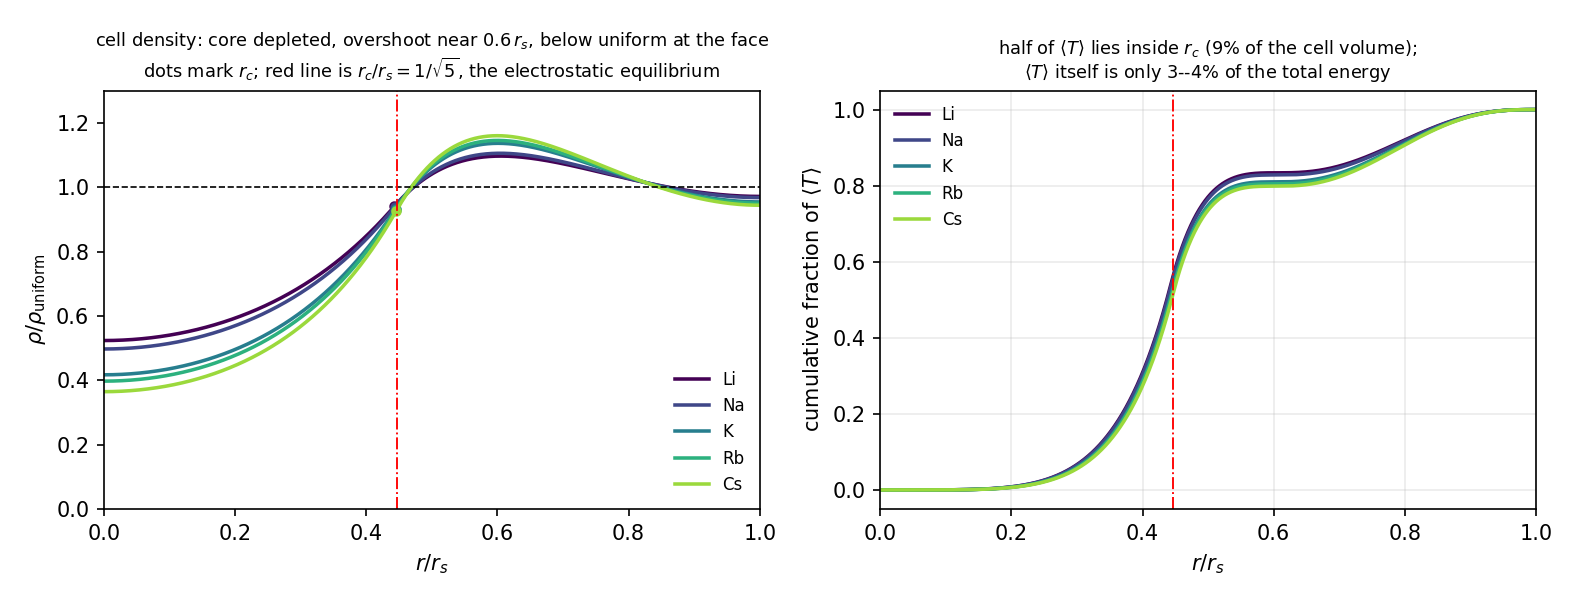
\includegraphics[width=\textwidth]{alkali_cell_density.png}
\end{center}

\noindent The five curves nearly coincide once lengths are measured in $r_s$, with
$r_c/r_s=0.443$--$0.446$, and that is not a coincidence. Minimising the electrostatic terms alone,
$-0.9/r_s + 1.5\,r_c^2/r_s^3$, gives
\[
  r_s=\sqrt5\,r_c,\qquad\text{so}\qquad r_c/r_s = 1/\sqrt5 = 0.4472 ,
\]
and the full calculation sits $+1.0,\,+0.9,\,+0.6,\,+0.5,\,+0.3\%$ from that closed form down the
group. So the equilibrium radius is fixed by the core radius to within one per cent, and
$\langle T\rangle$ --- which is $2.7$ to $4.2\%$ of the total energy --- supplies only that last per
cent. \emph{This must temper what the example is taken to show.} It demonstrates the route: a
macroscopic coefficient obtained by differentiating a computed energy, with nothing averaged and no
limit taken. It is a poor discriminator \emph{between theories}, because the quantity it reports is
set by the core radius and not by the kinetic term, which is the only ingredient separating RealQM
from the standard treatment here. The modulus, being a second derivative, separates them somewhat
better than the radius does. A system in which $\langle T\rangle$ carried a larger share of the
energy would test the construction harder, and the series does not.

\paragraph{What the comparison does and does not show.} On equal input the two treatments are
\emph{level}: at the claimed level RealQM is slightly the better on the modulus, $13\%$ against
$14\%$, and slightly the worse on the equilibrium radius, $5.1\%$ against $4.3\%$. We say this
plainly because an earlier draft of this work claimed more. Taking $r_c$ from the Ashcroft
literature instead, one radius per element, RealQM comes out ahead on both --- $1.2\%$ against
$4.1\%$ in $r_s$ and $17\%$ against $28\%$ in $B$ --- and its error then falls monotonically down the
group, reaching zero at caesium, which the standard column's does not. \emph{Neither of those
survives determining $r_c$ inside the theory.} The ordering by atomic number is not reproduced at
either level above, and the advantage becomes a tie. Both were properties of the literature radii,
which are themselves fitted within the standard pseudopotential framework and are not a neutral
input; a RealQM advantage measured against them was measuring the fit. What survives is weaker and
worth more: macroscopic material constants, to five and fifteen per cent, from Coulomb geometry with
one constant, obtained without averaging and with no ingredient the theory did not already have.

\emph{The literature radii, and lithium.} Those radii are not used above, and should not be: with
them lithium's modulus comes out $4.3$ times too stiff, which is the whole of the $79\%$ series
error that choice carries. The diagnosis is available. Fitting the empty core to the free atom gives
radii a nearly constant $12\%$ above the literature's for Na, K, Rb, Cs and $62\%$ above it at
lithium; and the two core models of the previous paragraph, each fitted to the same ionization
energy, stand in the ratio $r_c/R = 0.858,\,0.863,\,0.855,\,0.852,\,0.847$ --- a constant $0.855$
with a standard deviation of $0.006$ in which lithium is \emph{not} an outlier, though against the
literature radii it is. Lithium's anomaly therefore belongs to the tabulated radius, not to this
construction, which is why determining $r_c$ internally removes it rather than repairing it.

\emph{What the core radius does not reach.} Lithium's pressure derivative is not repaired by any of
this: $B'$ moves from $-0.71$ at the literature radius to $-0.21$, six times smaller in magnitude but
still the wrong sign, and the other four elements barely move. The modulus at lithium was an input
error; $B'$ fails for the separate reason identified in~\S\ref{sec:form} --- the order of the
derivative taken --- and no choice of core radius addresses that.

\emph{The constant is monovalent.} Carried to divalent magnesium it does not transfer: the same
construction, one electron on a $+1$ kernel matched to the first ionization energy, gives
$r_c=0.813$ against the literature's $1.39$, low by $42\%$. A valence-matched pseudo-atom --- a $+2$
kernel with two electrons and the self-repulsion reduced by $\tfrac12$, matched to the sum of the
first two ionization energies --- gives $1.291$, low by $7\%$, which is far better but is a different
construction on which no constant was calibrated. One constant for all therefore holds within a
valence column, and whether each column has its own is open.

Three things should be kept attached to the tables. At the level we claim, the calculation's entire
freedom is one constant fixed by one measured number, with each element's ionization energy supplying
the rest; at the level above it there is no fitted constant at all, and the departure is
one-sided, every radius high by about $11\%$, which is the atom-to-solid core contraction and not
scatter. A bulk modulus is a second derivative, so it amplifies the model's error in the way
H$_2$'s binding energy amplifies the error on its total --- which is why the percentages are large
where they are large. And agreement quoted to two figures means agreement to the two or three
significant figures the measured values carry, not exactness. What the table establishes is that
macroscopic material constants follow from Coulomb geometry across a series in which $r_s$ varies by
$70\%$ and $B$ by a factor of six --- obtained without averaging, with no ingredient the theory did
not already have, and varying with the element in a way the theory did not get to choose.

\section{The route checked against the mechanics it bypasses}\label{sec:checks}

The objection to \eqref{eq:modulus} is not that the energy is hard to compute but that differentiating it
\emph{bypasses} the mechanics: no stress is ever formed, so nothing guarantees that the number
differentiated is the number a force balance would have produced. That is now checked, and it had
to be, because the two are the same physics.

\paragraph{The stress, written down.} With $u=\sqrt\rho$ and $Q=-\tfrac12\grad^2u/u$, the chain rule
alone gives
\begin{equation}\label{eq:stress}
\rho\,\grad Q \;=\; \grad\cdot T,\qquad
T_{ij} \;=\; -\tfrac12\big[\,u\,\partial_i\partial_j u - \partial_i u\,\partial_j u\,\big]
\;=\; -\tfrac14\partial_i\partial_j\rho + \frac{\partial_i\rho\,\partial_j\rho}{4\rho},
\end{equation}
with no $\delta_{ij}$ term; in one dimension this is $\sigma=\tfrac14[(\rho')^2/\rho-\rho'']$. The
static Euler--Lagrange equation of the model is $Q+V=\lambda$ with $V=-K+P_{\rm other}$, so the
$v=0$ momentum balance is the statement
\begin{equation}\label{eq:divT}
\grad\cdot T \;=\; -\rho\,\grad V ,
\end{equation}
and integrating its $z$-component over a half space $\{z>z_{\rm cut}\}$ turns it into a statement
about forces: the flux of quantum stress through the cut equals the net electrostatic force on the
charge beyond it. The left-hand side is a surface integral of a quantity carrying a \emph{third}
derivative of the density; the right-hand side is a volume integral of Coulomb forces. Nothing makes
them equal except the identity.


Equation~\eqref{eq:divT} is a stress balance the model satisfies pointwise, with no averaging and
no approximation beyond the chain rule. It is the statement to be checked against.

Take the one-dimensional analogue of the cell construction above: a chain of period $a$,
one kernel of charge $+1$ and one electron per cell, each electron on its own cell with the free
interfaces at the cell faces by symmetry --- RealQM's non-overlap, and the same prescription the
sodium calculation uses. In equilibrium the total momentum flux through any plane is the same
number, and that number is the pressure. So the pressure and the modulus can each be computed twice,
once by differentiating the energy and once from the stress,
\[
\sigma \;=\; \underbrace{T_{zz}(\text{face})}_{\text{localisation stress}}
 \;+\; \underbrace{F_{\rm Coul}(\text{face})}_{\substack{\text{electrostatic force of everything left}\\ \text{of the face on everything right}}}
\quad\text{against}\quad -\frac{dE}{da},
\qquad
a\frac{d\sigma}{da}\quad\text{against}\quad a\frac{d^2E}{da^2},
\]
with no ingredient shared between the two sides beyond the converged ground state. They agree, and
the agreement improves under refinement:
\begin{center}
\begin{tabular}{lrrrrr}
\toprule
relative difference & $n=41$ & $n=61$ & $n=81$ & $n=101$ & extrapolated \\
\midrule
pressure, $\sigma$ against $-dE/da$        & $2.3\%$ & $1.6\%$ & $1.2\%$ & $0.96\%$ & $2.2\times10^{-4}$ \\
modulus, $a\,d\sigma/da$ against $a\,d^2E/da^2$ & $3.3\%$ & $2.2\%$ & $1.6\%$ & $1.3\%$ & $4.5\times10^{-4}$ \\
\bottomrule
\end{tabular}
\end{center}

Two features of the convergence are worth recording. It is \emph{first order} in the mesh, and the
reason is the one Section~\ref{sec:balance} draws out: the stress is evaluated \emph{at} the free
interface, where this construction is first-order accurate although it is fourth-order in the bulk.
The free boundary is again the accuracy-limiting feature. And neither lattice sum is responsible ---
the Coulomb flux is converged by the sixth neighbour and the lattice energy by the tenth, because
both are summed as \emph{neutral} cells, each of which is inversion symmetric about its kernel and
therefore carries no dipole, leaving a quadrupolar $1/d^3$ tail. Summed term by term the
one-dimensional Coulomb sums diverge logarithmically; summed as neutral units they converge at once.

What this establishes is modest and worth having: the scalar that \eqref{eq:modulus} differentiates
is the scalar a stress balance returns. The direct route is a shortcut through the mechanics, not a
detour around it.

\paragraph{The form, verified, and where the route's accuracy actually runs out.}\label{sec:form} The objection
to \eqref{eq:modulus} that cannot be answered by computing more coefficients is that it presupposes
the \emph{form}: $E$ quadratic in the strain, which is Hooke's law put in rather than derived. The
programme's answer is to establish the form computationally, and that has now been done, with a
result sharper than expected in one direction and worse in another.

On the periodic chain, straining the cell about a reference state and fitting a quadratic on
$|\epsilon|\le0.05$ alone, the energy then \emph{extrapolates} as a quadratic out to about
$|\epsilon|\approx0.06$ within $5\%$ of the quadratic term, with the cubic contribution rising
smoothly to $10\%$ at $|\epsilon|=0.10$ and $20\%$ at $0.22$. So the quadratic form is not assumed
but observed, over a range of strain, with the departure appearing where anharmonicity should.

The quantitative version of the same test is less kind, and it bounds the direct route in a way
worth stating. The cubic coefficient is not a free shape parameter: it fixes $B'=dB/dP$, the
pressure derivative of the bulk modulus, which is measured and which for the alkalis is close
to~$4$. Computed from the same energy curves that gave the table above, by finite differences and
with no equation of state fitted, the model returns
\[
B' \;=\; -0.71,\; 0.10,\; 1.35,\; 1.92,\; 2.63 \qquad\text{for Li, Na, K, Rb, Cs,}
\]
against a measured value near $4$ throughout. The familiar monotone improvement down the group is
there again, and caesium is again the best, but even caesium is a third low and lithium comes out
with the wrong sign --- a bulk modulus that \emph{falls} under pressure, which no alkali does.

The lesson is not that the route fails but that its accuracy is bounded by the \emph{order of the
derivative} rather than by the kind of coefficient. The energy of these cells is good to a few per
cent, the first derivative gives equilibrium densities to about one per cent for the heavy alkalis,
the second gives bulk moduli to ten or twenty per cent, and the third is gone. The claim above, that this route reaches
every coefficient which is a derivative of an energy, should be read with that ladder attached, because each differentiation spends accuracy the model does not have to spare.

\paragraph{Reaching a body, and the one quantity that needs no scale separation.} Coefficients are
not yet the statics of an elastic body. For that one needs a macroscopic stress field $\sigma(x)$
over the body, hence that the material at each point behaves like a uniformly strained cell --- the
\emph{Cauchy--Born} hypothesis. Granted it, elastostatics follows in the ordinary way: minimise
$\int_\Omega W(\epsilon(u))\,dx$ less the work of the loads, with $W$ the cell energy computed above,
and the Euler--Lagrange equation of that functional is $\grad\cdot\sigma=f$ with the given boundary
conditions. Nothing further is required of RealQM. But Cauchy--Born is assumed here, exactly as
$\varepsilon\ll1$ is assumed in \eqref{eq:eps}, and it is known to fail at surfaces, defects and
crack tips --- which is to say at most of the problems elasticity is wanted for.

That failure is where this formulation has an advantage rather than a handicap. In a lattice model a
surface can only be made by truncating the lattice. Here a surface \emph{is} a free boundary, the
object the theory is built on, and a surface energy is therefore a difference of computed energies
needing no scale separation at all. On the finite chain, with the interior interfaces at the cell
midpoints and the two end domains left to run out into vacuum and find their own extent,
$E(N)=N\,e_{\rm bulk}+2\gamma$ gives
\[
\gamma = 0.0416~\text{Ha} = 1.13~\text{eV per end},
\]
and the test that makes this a surface property rather than a fitted intercept is that $\gamma$ is
\emph{independent of} $N$ --- flat to $3\times10^{-7}$ from $N=5$ onwards. It converges at second
order in the mesh, and the bulk energy read off the finite chains agrees with the periodic
calculation, computed by different code, also at second order. So the free boundary carries a
surface energy, it is stable against the size of the system, and it was obtained without the
hypothesis that the rest of the elastic programme rests on.

\section{Why it works: the model is already a continuum mechanics}\label{sec:balance}

The agreement just recorded is not a coincidence of this discretisation, and it is worth saying
why before the limits are drawn. Differentiating a scalar reproduced a force balance to
$2\times10^{-4}$ because the model was a continuum mechanics before any upscaling was attempted.
Two identities show it, and both are the chain rule.

\paragraph{The localisation energy is the von Weizs\"acker functional.} Writing
$\rho_i=\psi_i^2$ with $\psi_i\ge0$, the chain rule gives $\grad\rho_i = 2\psi_i\grad\psi_i$, hence
\begin{equation}\label{eq:vW}
\half\int|\grad\psi_i|^2\,dx \;=\; \frac18\int\frac{|\grad\rho_i|^2}{\rho_i}\,dx
\;=\; T_{\rm vW}[\rho_i] ,
\end{equation}
in units $\hbar=m=1$. An identity, not a model.

\paragraph{Its variation is the quantum potential.} With $u=\sqrt{\rho}$,
\begin{equation}\label{eq:Q}
\frac{\delta T_{\rm vW}}{\delta\rho} \;=\; -\half\frac{\grad^2\sqrt{\rho}}{\sqrt{\rho}} \;=\; Q ,
\end{equation}
Bohm's quantum potential --- obtained here not by analogy but as the variation of a term
\eqref{eq:E} writes down for an unrelated reason, namely the cost of confining a charge to a region.

\paragraph{The theory as used is a hydrostatics.} Stationarity of \eqref{eq:E} is the statement that
$V+Q$ is constant on each domain, which is the $v=0$ case of the Madelung pair
\begin{align}
\frac{\partial\rho}{\partial t}+\grad\!\cdot(\rho v)&=0 ,\label{eq:cont}\\
\frac{\partial v}{\partial t}+(v\cdot\grad)v&=-\grad\bigl(V+Q\bigr) .\label{eq:euler}
\end{align}
Equation~\eqref{eq:cont} is conservation of charge and \eqref{eq:euler} is a momentum balance whose
stress is supplied by \eqref{eq:Q}. \emph{RealQM is therefore already the equilibrium of a continuum
mechanics, and the constitutive law is not postulated --- it is the variation of the energy the
theory was written with.} This is the sense in which the derivation asked for by Hilbert is, on this
route, partly a matter of recognition rather than of proof.

That is why the two-route check had to succeed: it compared two readings of one balance, not two
theories. It also places the free interfaces, which carry an energy per unit area and so make this a
continuum mechanics \emph{with surfaces} --- what dense matter requires, and what a kinetic theory
has no room for~\cite{madelung}. The surface energy computed above is that term.

\section{Where the direct route stops}\label{sec:stops}

\paragraph{And where it stops, which is the informative part.} The direct route reaches a
coefficient if and only if that coefficient is a derivative of an energy. \emph{Viscosity is not.} A
viscous stress is dissipative: the work done against it is not stored, so there is no
$E(\text{strain rate})$ to differentiate, and no variational principle whose minimiser contains
$\eta$. This is exactly why the standard treatment reaches for Green--Kubo, which extracts a
transport coefficient from equilibrium fluctuations and therefore needs an ensemble.

So the division of the problem is sharp, and it is not an artefact of the method chosen:
\begin{center}
\begin{tabular}{lll}
\toprule
 & conservative coefficients & dissipative coefficients \\
\midrule
examples    & elastic tensor, $P(V)$, phonons & viscosity, thermal conductivity \\
nature      & derivative of ground-state energy & transport, no energy functional \\
this route  & \textbf{direct, no averaging} & \textbf{not reached} \\
\bottomrule
\end{tabular}
\end{center}

Equilibrium continuum mechanics follows from RealQM by differentiating computed energies.
Dissipation does not follow at all, and is the whole of what remains open
(Section~\ref{sec:stops}).

\paragraph{What is given up, stated plainly.} The direct route delivers the \emph{coefficients} of
the macroscopic laws, not their \emph{form}. Writing \eqref{eq:modulus} presupposes that $E$ is
quadratic in the strain near equilibrium --- that is, it assumes Hooke's law rather than deriving
it. Homogenisation would instead produce linear elasticity as the macroscopic limit, form and
coefficient together, and that is a genuine advantage of the formal route which should not be
waved away.

Two things reduce the force of the objection. The form can be established computationally: compute
$E(\epsilon)$ across a range and verify that it is quadratic, and that the departure from quadratic
sets in where nonlinear elasticity is observed to set in. That is a demonstration and not a theorem.
And a demonstration is the kind of evidence this programme is built to give --- its standing claim is
that its assertions are testable \emph{because} computable, and reaching instead for an asymptotic
theorem would borrow precisely the sort of authority it declines to grant to the standard formalism
elsewhere. The formal route remains worth having; it is not what the next computation should wait
for.

\begin{thebibliography}{9}

\bibitem{DHM2025} Y.~Deng, Z.~Hani and X.~Ma, \emph{Hilbert's sixth problem: derivation of fluid
equations via Boltzmann's kinetic theory}, arXiv:2503.01800 (2025).

\bibitem{Comment2025} \emph{Comment on ``Hilbert's Sixth Problem: Derivation of Fluid Equations via
Boltzmann's Kinetic Theory'' by Deng, Hani and Ma}, arXiv:2504.06297 (2025).

\bibitem{madelung} C.~Johnson, \emph{The Hydrodynamic Form of RealQM: Madelung Hydrostatics, a
Surface Tension, and the Missing Half}.

\bibitem{realqm} C.~Johnson, \emph{RealQM: Quantum Mechanics as Multiphase 3D Continuum Mechanics},
in~\cite{realqmbook}.

\bibitem{realqmbook} C.~Johnson, \emph{Real Quantum Mechanics} (Body\&Soul, Vol.~VI),
\url{https://claes542.github.io/RealMolecule/realquantum3.pdf}.

\bibitem{gas} C.~Johnson, \emph{Conduction in RealQM: the Free Boundary as Charge Carrier},
in~\cite{realqmbook}.

\bibitem{nomass} C.~Johnson, \emph{Energy without Mass: the Kinetic Coefficient as a Geometric
Scale, and Inertia as $E/c^2$}.

\bibitem{bodysoul} C.~Johnson, \emph{Computational Thermodynamics} (Body\&Soul, Vol.~V).

\bibitem{hilbert6} C.~Johnson, \emph{Upscaling of RealQM towards
Hilbert's Sixth Problem}, companion paper.

\bibitem{atoms} C.~Johnson, \emph{RealQM for Atoms and the Periodic Table}.

\bibitem{clay} C.~Johnson, \emph{The Clay Navier--Stokes Problem and Computational
Well-Posedness}.

\end{thebibliography}

\end{document}
